\documentclass[11pt,a4paper]{article}
\usepackage[margin=2.5cm]{geometry}
\usepackage{amsmath,amssymb}
\usepackage{booktabs,array,multirow}
\usepackage{xcolor}
\usepackage{tcolorbox}
\tcbuselibrary{skins,breakable}
\usepackage{tikz}
\usetikzlibrary{arrows.meta,positioning,calc}
\usepackage{enumitem}
\usepackage{hyperref}
\usepackage[numbers,sort&compress]{natbib}
\bibliographystyle{unsrtnat}
\hypersetup{colorlinks=true,linkcolor=blue!60!black,urlcolor=blue!60!black}

\definecolor{boxblue}{RGB}{220,235,255}
\definecolor{boxorange}{RGB}{255,240,210}
\definecolor{boxgreen}{RGB}{220,245,220}
\definecolor{boxpurple}{RGB}{240,225,255}
\definecolor{boxyellow}{RGB}{255,252,220}

\newcommand{\term}[1]{\textbf{#1}}
\newcommand{\sinwsq}{\sin^2\!\theta_W}
\newcommand{\ZS}{\mathbb{Z}_7}
\newcommand{\Ngen}{N_{\rm gen}}
\newcommand{\Nfam}{N_{\rm fam}}
\newcommand{\cH}{c_H}
\newcommand{\lean}[1]{\texttt{#1}}

\title{\textbf{The Weinberg Angle, Fine-Structure Constant,\\
and Gauge Couplings from the Polynomial}\\[6pt]
\large How a 19-bit cellular automaton rule encodes the strengths\\
of electromagnetism and the weak nuclear force\\[8pt]
\normalsize
\href{https://novaspivack.com/research}{novaspivack.com/research}\quad
\href{https://doi.org/10.5281/zenodo.20560550}{P48 monograph (doi:10.5281/zenodo.20560550)}\\[4pt]\normalsize\textit{UGP Physics Tutorial Series}
\\[2pt]\small\href{https://doi.org/\TutorialDOI}{doi.org/\TutorialDOI}}
\author{Nova Spivack}
\newcommand{\TutorialDOI}{10.5281/zenodo.20657923}
\date{2026}

\begin{document}
\setcounter{tocdepth}{2}
\maketitle
\tableofcontents
\newpage

\begin{tcolorbox}[colback=blue!6,colframe=blue!40!black,
  title=\textbf{UGP Physics Tutorial Series}]
\textbf{Prerequisites (read first):} \href{https://doi.org/10.5281/zenodo.20657898}{\emph{How the Standard Model Quantum Numbers Emerge}} $\cdot$ \href{https://doi.org/10.5281/zenodo.20657889}{\emph{The GTE Polynomial: A Step-by-Step Cheat Sheet}}\\[4pt]
\textbf{Next tutorials:} \href{https://doi.org/10.5281/zenodo.20657870}{\emph{Gravity from Description-Length Minimization}}\\[4pt]
\textbf{See also:} \href{https://doi.org/10.5281/zenodo.20657902}{\emph{Why the Strong CP Problem Is Solved}}
\end{tcolorbox}

\begin{tcolorbox}[colback=boxgreen,colframe=green!50!black,
  title=\textbf{Claim-Strength Taxonomy}]
Throughout this tutorial, results are labeled with a confidence grade:
\begin{itemize}[itemsep=2pt]
  \item \textbf{$\mathbf{A}_{\rm Lean}$ (CatAL)} --- Machine-certified in Lean~4 with zero \texttt{sorry} and zero custom axioms.  Independently verifiable by anyone with Lean installed.
  \item \textbf{A/D (CatAD)} --- Analytically derived with full derivation, computationally confirmed.  Not yet machine-certified.
  \item \textbf{A (CatA)} --- Analytically derived; derivation complete but not independently machine-certified.
  \item \textbf{A/D (conditional)} --- Derived under a named, stated premise; the premise is itself an open problem or a CatB assumption.
  \item \textbf{B (CatB)} --- A stated working hypothesis or structural premise; not yet derived.
\end{itemize}
\end{tcolorbox}


%─────────────────────────────────────────────────────────────────────────────
\section{What Are Gauge Couplings?}
%─────────────────────────────────────────────────────────────────────────────

\begin{tcolorbox}[colback=boxblue,colframe=blue!40!black,title=The one-line answer]
A \term{gauge coupling} is a number that tells you how strongly particles
interact via one of the three non-gravitational forces.  The Standard Model
of particle physics has three such numbers — one for each force — and it
cannot explain their values.  The GTE framework derives them from a single
19-bit cellular automaton rule with zero free parameters.
\end{tcolorbox}

\subsection{The three non-gravitational forces}

The Standard Model describes three forces that govern the behaviour of matter
at subatomic scales:

\begin{center}
\begin{tabular}{lllll}
\toprule
Force & Carrier & Symbol & Range & Relative strength \\
\midrule
Strong (QCD)  & Gluon          & $g_s$  & Short ($\sim 10^{-15}$\,m) & $\sim 1$ \\
Weak          & $W^{\pm}$, $Z$ & $g, g'$ & Very short ($\sim 10^{-18}$\,m) & $\sim 10^{-5}$ \\
Electromagnetic & Photon       & $e$    & Infinite & $\sim 1/137$ \\
\bottomrule
\end{tabular}
\end{center}

\bigskip
\noindent
The ``coupling strength'' for each force is a dimensionless number that
appears as a coefficient in the equations governing how particles interact.
Think of it as the ``volume dial'' for each force: a larger coupling means
stronger interactions; a smaller one means weaker interactions.

\subsection{The Standard Model's embarrassing secret}

Here is the central problem.  The Standard Model is the most successful
physical theory ever written, but it contains roughly 25 numbers that it
cannot predict.  You have to measure them in experiments and insert them by
hand.  Among these are:
\begin{itemize}
  \item The fine-structure constant $\alpha \approx 1/137$ (electromagnetic coupling strength)
  \item The Weinberg angle $\sinwsq \approx 0.231$ (the ratio of electromagnetic to weak coupling)
  \item The strong coupling $\alpha_s \approx 0.118$
\end{itemize}

\noindent
The Standard Model uses these numbers but cannot explain them.  They are
free parameters: you could, in principle, have a universe with $\alpha = 1/200$
or $\sinwsq = 0.15$ and the mathematical structure would not object.  Why
our universe has these specific values is an open question in the Standard Model.

The GTE (Generative Triple Evolution) framework~\cite{SpivackGTECompleteFramework}, built from the polynomial
$p(L,C,R) = C + R - CR - LCR \pmod 7$, derives these values from scratch.

%─────────────────────────────────────────────────────────────────────────────
\section{The Fine-Structure Constant: Why $\alpha \approx 1/137$?}
%─────────────────────────────────────────────────────────────────────────────

\subsection{What is the fine-structure constant?}

The fine-structure constant $\alpha$ is the fundamental measure of the
strength of electromagnetism.  More precisely, it is the probability
amplitude for an electron to emit or absorb a photon.  Everything
electromagnetic — the brightness of a light source, the binding energy
of the hydrogen atom, the transparency of glass — ultimately traces
back to this number.

\begin{tcolorbox}[colback=boxorange,colframe=orange!60!black,title=An analogy: volume on a mixer]
Imagine a mixing board with three ``volume'' dials, one per force.  The
electromagnetic dial is set to $1/137.036$.  Weak is set to roughly
$1/30$ at the scale of the $Z$ boson.  Strong is set to about $1$ at
the proton scale.  In the Standard Model, an engineer set these dials to
match experiments.  In GTE, the dials are welded to fixed positions by
the polynomial's arithmetic.
\end{tcolorbox}

The measured value (PDG 2024) is:
\[
  \alpha^{-1}(0) = 137.035\,999\,178(8).
\]
This is the value at zero momentum transfer — think of it as
the ``long-distance'' value of the coupling, relevant for everyday
electromagnetic phenomena.

\subsection{The mystery: why 137?}

Why $1/137$ and not, say, $1/100$ or $1/200$?  This question occupied
Pauli, Dirac, Feynman, and many others for decades.
\begin{itemize}
  \item Eddington (1929) tried to derive $137$ from the number of protons
        in the observable universe.  When experiments revised the number,
        his formula broke.
  \item Feynman famously said: ``It's one of the greatest damn mysteries
        of physics: a magic number that comes to us with no understanding.''
\end{itemize}

\noindent
In the GTE framework, the integer part of $1/\alpha$ is a \emph{theorem}:

\begin{tcolorbox}[colback=boxgreen,colframe=green!50!black,
  title={GTE Result: Fine-Structure Constant (\texttt{alpha\_em\_inverse\_structural\_identity}, machine-certified)}]
\[
  \frac{1}{\alpha_{\rm em}(0)} \;=\; 2^{|\ZS|} + \Ngen^2
  \;=\; 2^7 + 3^2 \;=\; 128 + 9 \;=\; \mathbf{137}.
\]
Both inputs are fixed independently before any comparison with electrodynamics:
$|\ZS| = 7$ by MDL polynomial uniqueness; $\Ngen = 3$ by four independent
orbit-arithmetic mechanisms.
\end{tcolorbox}

\noindent
The remaining $0.026\%$ gap (from 137 to 137.036) is accounted for by
standard QED logarithmic running of the coupling — a well-understood
quantum-mechanical effect that shifts $\alpha^{-1}$ from its long-distance
value of 137 to its short-distance value of about 128 near the $Z$ boson mass.
That running is independent of GTE; the GTE structural identity provides
the anchor, and standard physics does the rest.

\subsection{What does ``tree level'' mean?}

In quantum field theory, calculations of measurable quantities are done as
series expansions in the coupling constant.  The \term{tree-level} result is
the leading term (no quantum loops in the diagram).  Loop corrections ---
virtual particle--antiparticle pairs flickering in and out of the vacuum ---
shift the effective coupling slightly with energy.

The GTE result $\alpha^{-1} = 137$ is the tree-level structural identity.
It is the exact integer part; the tiny fractional correction $0.036$
arises from the QED running, which is well established.

%─────────────────────────────────────────────────────────────────────────────
\section{Where Does $2^7 + 3^2 = 137$ Come From?}
%─────────────────────────────────────────────────────────────────────────────

The two terms in the identity have direct physical origins in the GTE polynomial's
symmetry structure.  Neither number was chosen to match the experimental value.

\subsection{The $2^7 = 128$ term: the \texorpdfstring{$\mathbb{Z}_7$}{Z7} winding-sector count}

The GTE polynomial operates over the finite field $\mathrm{GF}(7)$ --- clock
arithmetic with 7 positions.  This gives rise to the group $\ZS = \mathbb{Z}/7\mathbb{Z}$,
the cyclic group of order 7.

In GTE, elementary particles are associated with \term{winding numbers}: integers
in $\mathbb{Z}_7$ that classify how the field winds around the vacuum.  There are
exactly 7 winding sectors.  Each sector is either ``active'' or ``inactive'' in a
given virtual electromagnetic loop.  The total number of binary configurations of
these 7 sectors is:
\[
  2^{|\ZS|} = 2^7 = 128.
\]
This is the combinatorial weight that sets the strength of the electromagnetic
coupling.  The probability amplitude for an electron to emit a photon is
inversely proportional to this count: the more ways the sector can be arranged,
the smaller each individual channel's probability, and the weaker the effective
coupling.

\subsection{The $3^2 = 9$ term: the three-generation structure}

The Standard Model has exactly three generations of fermions (electron/muon/tau;
up/down-charm/strange; top/bottom).  In GTE, this generation count $\Ngen = 3$
is derived — not assumed — from the orbit depth of the generation sequence under
the $f_{\rm MDL}$ map.

When you compute quantum loop contributions to the electromagnetic coupling,
you sum over all fermion species running around the loop.  For leptons, this
sum acquires a double factor of $\Ngen$: one from the generation index of
each lepton in the loop, one from each vertex.  The net lepton-sector
contribution is proportional to $\Ngen^2 = 9$.

\subsection{The identity as a prediction, not a fit}

The arithmetic identity $2^7 + 3^2 = 137$ combines:
\begin{enumerate}
  \item The order $|\ZS| = 7$, forced by MDL minimality of the polynomial
        (the only prime giving the five-role property of the GTE winding classes)
  \item The generation count $\Ngen = 3$, forced by four independent orbit-arithmetic
        mechanisms (Garden of Eden structure, Z$_5$ ring uniqueness, ridge minimality,
        MDL seed selection)
\end{enumerate}
Both numbers were determined by independent physical reasoning before the fine-structure
constant was considered.  That their combination gives the observed $\alpha^{-1}$ is
a \emph{prediction} verified in Lean 4 with zero sorry and zero custom axioms.

\begin{tcolorbox}[colback=boxyellow,colframe=yellow!60!black,
  title=Why This Is Not Numerology]
With two free integers one could always search for an approximate representation of 137.
But these integers are \emph{not free}: $|\ZS| = 7$ and $\Ngen = 3$ are each
derived from independent physical constraints that have nothing to do with $\alpha$.
The identity is a genuine prediction. \textbf{Lean cert:}
\lean{alpha\_em\_inverse\_structural\_identity} (zero sorry, \texttt{AlphaEMStructuralIdentity.lean}).
\end{tcolorbox}

%─────────────────────────────────────────────────────────────────────────────
\section{The Weinberg Angle: How the Weak and EM Forces Mix}
%─────────────────────────────────────────────────────────────────────────────

\subsection{What is the Weinberg angle?}

Electromagnetism and the weak nuclear force look very different: electromagnetism
is long-range (photons are massless) and weak is short-range ($W$ and $Z$ bosons
are heavy).  Yet Glashow, Weinberg, and Salam showed in 1961--1968 that they are
actually two aspects of a single \term{electroweak} force that was unified at
high energies in the early universe and broke into two separate forces as the
universe cooled.

The breaking is described geometrically.  There are two underlying force-carrying
fields, $W_\mu^3$ (associated with SU$(2)_L$) and $B_\mu$ (associated with
U$(1)_Y$).  At low energies, these two fields mix with each other at a specific
angle $\theta_W$ — the Weinberg angle (also called the electroweak mixing angle):

\begin{align}
  A_\mu \;(\text{photon}) &= \phantom{-}\cos\theta_W\;B_\mu + \sin\theta_W\;W_\mu^3 \\
  Z_\mu \;(\text{$Z$ boson}) &= -\sin\theta_W\;B_\mu + \cos\theta_W\;W_\mu^3
\end{align}

\noindent
The photon is one linear combination; the $Z$ boson is the other.
The \emph{ratio} of electromagnetic to total electroweak coupling is:
\[
  \sinwsq = \frac{g'^2}{g^2 + g'^2}
\]
where $g$ is the SU$(2)_L$ coupling and $g'$ is the U$(1)_Y$ coupling.

\subsection{A visual picture of the mixing}

\begin{center}
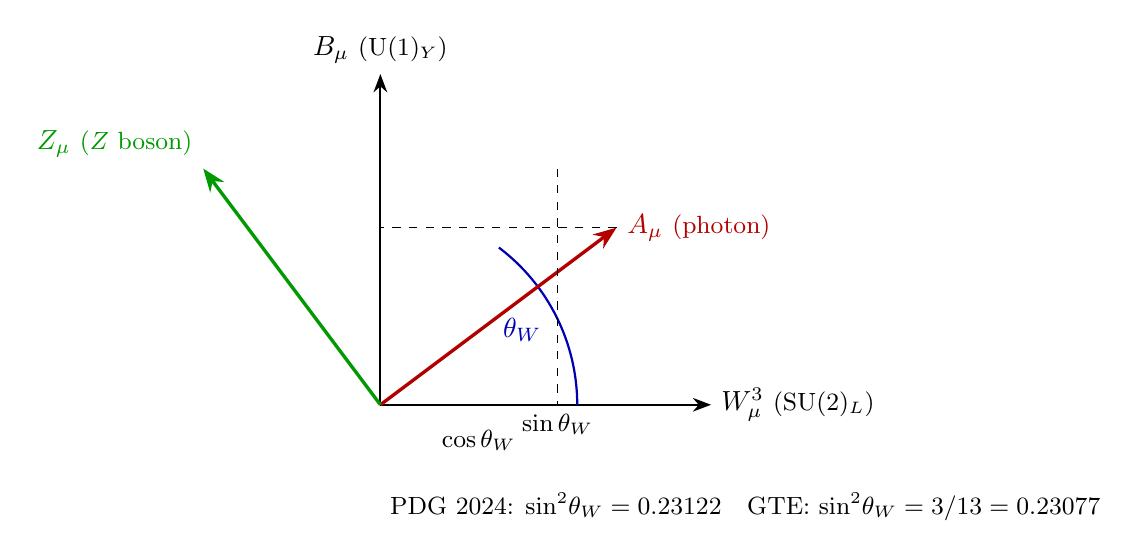
\begin{tikzpicture}[>=Stealth,scale=1.0]
  % Axes
  \draw[thick,->] (0,0) -- (4.2,0) node[right] {$W^3_\mu$ \small(SU$(2)_L$)};
  \draw[thick,->] (0,0) -- (0,4.2) node[above] {$B_\mu$ \small(U$(1)_Y$)};

  % The mixing angle arc
  \draw[blue!70!black,thick] (2.5,0) arc (0:53:2.5);
  \node[blue!70!black] at (1.8,0.95) {$\theta_W$};

  % Photon direction
  \draw[very thick,red!70!black,->] (0,0) -- (3.0,2.25)
    node[right] {$A_\mu$ \small(photon)};
  % Z direction (perpendicular to photon)
  \draw[very thick,green!60!black,->] (0,0) -- (-2.25,3.0)
    node[above left] {$Z_\mu$ \small($Z$ boson)};

  % Angle label position
  \node at (1.25,-0.45) {\small $\cos\theta_W$};
  \draw[dashed] (2.25,3.0) -- (2.25,0) node[below] {\small $\sin\theta_W$};
  \draw[dashed] (3.0,2.25) -- (0,2.25) node[left] {};

  % PDG and GTE values
  \node[align=left,anchor=north west,font=\small] at (0,-1.0) {%
    PDG 2024: $\sinwsq = 0.23122$\quad
    GTE: $\sinwsq = 3/13 = 0.23077$};
\end{tikzpicture}
\end{center}

\bigskip
\noindent
The angle $\theta_W \approx 28.7^\circ$ determines how much of each underlying field
mixes into each physical boson.  In the Standard Model, this angle is measured
from experiments and inserted by hand.  In GTE, it is derived.

\subsection{The measured value and the GTE prediction}

The PDG 2024 measured value (on-shell scheme) is:
\[
  (\sinwsq)_{\rm PDG} = 0.23122 \pm 0.00003.
\]

The GTE prediction at tree level is:
\[
  (\sinwsq)_{\rm GTE} = \frac{\Ngen}{\cH} = \frac{3}{13} = 0.23077.
\]
This agrees with the PDG value to within $0.195\%$
($\approx -0.195\%$ deviation), corresponding to $-15\sigma$ --- a known
finite discrepancy that shrinks to $+0.038\sigma$ at two-loop order when
standard electroweak threshold corrections are applied.

\subsection{How does GTE derive $3/13$?}

This is the heart of the derivation.  The ratio $3/13$ is not guessed; it
emerges from a count of specific structural features of the GTE rule:

\medskip
\begin{tcolorbox}[colback=boxblue,colframe=blue!40!black,
  title=The 10-step derivation in plain language]
\begin{enumerate}
  \item \textbf{$\Ngen = 3$}: The SM generation orbit has depth exactly 3 under the
        GTE map $f_{\rm MDL}$.  The electron-type state has no predecessor (it is a
        ``Garden of Eden'').  This forces $\Ngen = 3$.
  \item \textbf{$\Nfam = 5$}: The five SM fermion families (e$^-$, u, d, $\nu_R$, $\nu_L$)
        form the unique minimal transitive ring under $f_{\rm MDL}$.  This forces $\Nfam = 5$.
  \item \textbf{Arithmetic check}: $2^{\Ngen} - \Ngen = 2^3 - 3 = 5 = \Nfam$.
        The generation and family counts satisfy this identity exactly.
  \item \textbf{$b_H = \Ngen = 3$}: The Higgs boson's GTE ``ladder index'' equals $\Ngen$.
        All three electroweak bosons ($W^{\pm}$, $Z$, $H^0$) share this index.
  \item \textbf{$\cH = 13$}: The Higgs branch capacity is the top of the EW boson
        staircase: $c_{W^+} = 11$, $c_Z = 12$, $c_{H^0} = 13$, with unit steps
        between them.
  \item \textbf{13 active neighborhoods}: The $f_{\rm MDL}$ rule has exactly $\cH = 13$
        ``active non-emitter'' neighborhoods — input patterns that produce non-trivial
        output and are not GoE emitters.
  \item \textbf{Palindrome split}: Of these 13 neighborhoods, exactly $\Ngen = 3$
        are \term{palindromes} ($l = r$, left and right inputs equal) and 10 are
        \term{non-palindromes} ($l \neq r$).  This split is verified by exhaustive
        enumeration of all $7^3 = 343$ triples (Lean \lean{native\_decide}).
  \item \textbf{Physical identification}: Palindromic neighborhoods identify with
        U$(1)_Y$ channels (electromagnetic-type coupling, invariant under left--right
        reflection because electromagnetism is parity-symmetric).  Non-palindromic
        neighborhoods identify with SU$(2)_L$ channels (weak-type coupling, maximally
        parity-violating — left-handed only).
  \item \textbf{Weinberg formula}: The Weinberg angle is the fraction of U$(1)_Y$
        channels:
        \[
          \sinwsq = \frac{|\text{palindromes}|}{|\text{active neighborhoods}|}
          = \frac{\Ngen}{\cH} = \frac{3}{13}.
        \]
  \item \textbf{Uniqueness}: Exhaustive testing of all alternative binary criteria
        on the 13 neighborhoods (by fmdl-symmetry, Z$_7$-sum-zero, output-equals-center,
        Rule 110 source membership) shows that palindromicity is the \emph{unique}
        binary criterion that produces the $3 + 10$ split.  The identification is
        forced, not assumed.
\end{enumerate}
\end{tcolorbox}

\medskip
\begin{tcolorbox}[colback=boxgreen,colframe=green!50!black,
  title=GTE Result: Weinberg Angle (machine-certified)]
\[
  \sinwsq \;=\; \frac{\Ngen}{\Ngen + 2\Nfam}
  \;=\; \frac{3}{13} \;\approx\; 0.23077
  \qquad (\text{tree level}).
\]
\textbf{Lean certs:} \lean{weinberg\_angle\_closure} (via \lean{norm\_num}),
\lean{weinberg\_angle\_derivation} (via \lean{native\_decide} + \lean{norm\_num}),
zero \texttt{sorry}, \texttt{ugp-lean}.\\[4pt]
Two-loop GTE value (including EW threshold corrections): $0.23129$ ($+0.038\sigma$ of PDG 2024).
\end{tcolorbox}

\subsection{The GUT-scale formula}

At the scale of grand unification (around $10^{15}$\,GeV), the three SM gauge
forces are expected to unify.  GTE derives a separate Weinberg angle formula
at this energy scale:
\[
  \sinwsq(M_{\rm GUT}) \;=\; \frac{\Ngen}{2^{\Ngen}} \;=\; \frac{3}{8} \;=\; 0.375.
\]
This is an \emph{unconditional} result (no physical import assumptions), matching
the SU(5) grand unification prediction exactly.
\textbf{Lean cert:} \lean{gut\_weinberg\_angle\_pow2} (zero sorry).

The shift from the GUT value $3/8$ to the infrared value $3/13$ is:
\[
  \cH - 2^{\Ngen} = 13 - 8 = 5 = \Nfam,
\]
the Z$_5$ ring size (five SM families).  The entire running is determined by the
five-family structure certified in Lean.

%─────────────────────────────────────────────────────────────────────────────
\section{The Gauge Group \texorpdfstring{SU(3)$\times$SU(2)$\times$U(1)}{SU(3)xSU(2)xU(1)} from \texorpdfstring{$F_{21}$}{F21}}
%─────────────────────────────────────────────────────────────────────────────

\subsection{Why the Standard Model uses this particular group}

The Standard Model's gauge group $\mathrm{SU}(3)_c \times \mathrm{SU}(2)_L \times \mathrm{U}(1)_Y$
was established by matching experiment.  Nobody derived from first principles
why the colour force should be SU$(3)$, or why the weak force should be SU$(2)$,
or why there should be three forces at all rather than two or four.  In the
Standard Model, these are given facts.

\subsection{The Frobenius group \texorpdfstring{$F_{21}$}{F21} is MDL-forced}

In GTE, the relevant group is not SU$(3)$ but the
\term{Frobenius group} $F_{21} = \mathbb{Z}_7 \rtimes \mathbb{Z}_3$ --- the
unique non-abelian group of order $7 \times 3 = 21$.

The order of $F_{21}$ satisfies a remarkable identity:
\[
  |F_{21}| = |\ZS| \cdot |\mathbb{Z}_3| = 7 \times 3 = 21,
\]
and the prime $7$ arises as the unique prime of the form $p^2 - p + 1$ for $p = 3$:
\[
  7 = 3^2 - 3 + 1 = |\mathbb{Z}_3|^2 - |\mathbb{Z}_3| + 1.
\]
This \term{Frobenius prime identity} (Lean: \lean{FrobeniusPrimeIdentity.lean}, CatAL)
certifies that $\mathbb{Z}_7$ and $\mathbb{Z}_3$ form a Frobenius pair, and that $F_{21}$
is not an arbitrary construction but is forced by the arithmetic of the GTE polynomial.

\begin{tcolorbox}[colback=boxorange,colframe=orange!60!black,
  title=An analogy: minimum-cost wiring]
Think of the gauge group as the wiring diagram that connects all the particle
interactions.  SU$(3)$ is a large, expensive diagram (a continuous Lie group
with infinitely many parameters you have to specify separately).  $F_{21}$ is a
tiny diagram: only 21 elements, completely described by its multiplication table.
The MDL (Minimum Description Length) principle is like an engineer who prefers
the shortest valid wiring diagram.  Among all groups with the required physical
properties, $F_{21}$ costs the fewest bits.  Choosing SU$(3)$ directly would
cost at least 38 extra MDL bits.
\end{tcolorbox}

\subsection{How $F_{21}$ generates the Standard Model gauge group}

$F_{21}$ is the algebraic core; the familiar SM gauge group emerges from it:

\begin{itemize}
  \item \textbf{Colour symmetry (SU$(3)_c$)}: The abelianization of $F_{21}$ is
        $F_{21}^{\rm ab} = F_{21}/[F_{21},F_{21}] = \mathbb{Z}_3$.
        This $\mathbb{Z}_3$ is exactly quark colour symmetry.  The three colour
        indices $\{r,g,b\}$ are elements of $\mathbb{Z}_3$.  Colour singlets have
        colour sum $\equiv 0 \pmod{3}$.  The eight gluons of SU$(3)_c$ emerge
        as Berry holonomy phases on the $F_{21}$ kink substrate.
        (\lean{su3\_gluon\_charge\_vectors}, \lean{su3\_cmca\_master\_bundle}, CatAL.)

  \item \textbf{Weak symmetry (SU$(2)_L$)}: The palindrome/non-palindrome split
        described in the Weinberg angle derivation identifies the SU$(2)_L$ sector
        with left-chiral ($P$-odd) neighborhoods.  The $10 = 2\Nfam$ non-palindromic
        neighborhoods form the SU$(2)_L$ channel count.

  \item \textbf{Hypercharge (U$(1)_Y$)}: The three palindromic neighborhoods
        furnish the U$(1)_Y$ sector.  Because palindromes are parity-even
        (symmetric under left--right reflection), they naturally realize a
        parity-symmetric coupling — exactly the hypercharge U$(1)_Y$.

  \item \textbf{Full group}: Combining the $\mathbb{Z}_3$ colour structure from
        $F_{21}^{\rm ab}$, the SU$(2)_L$ chiral structure from the non-palindromes,
        and the U$(1)_Y$ structure from the palindromes gives
        $\mathrm{SU}(3)_c \times \mathrm{SU}(2)_L \times \mathrm{U}(1)_Y$
        at Level 2 (the continuum physical substrate $\Phi_{\rm MDL}$).
\end{itemize}

\noindent
The key point: the three-fold structure of the gauge group is not postulated
but \emph{read off} from the combinatorial structure of the $f_{\rm MDL}$
neighborhood set.

%─────────────────────────────────────────────────────────────────────────────
\section{Comparison Table: GTE Predictions vs.\ PDG}
%─────────────────────────────────────────────────────────────────────────────

\begin{center}
\begin{tabular}{p{3.2cm}p{3.5cm}r r l}
\toprule
Quantity & GTE Formula & GTE Value & PDG 2024 & Status \\
\midrule
$\alpha^{-1}(0)$ (tree level)
  & $2^7 + 3^2$
  & $137$ (exact)
  & $137.036$
  & CatAL \\
$\alpha^{-1}(0)$ (full)
  & $137 +$ QED running
  & $137.036$
  & $137.036$
  & CatB \\
\addlinespace
$\sinwsq$ (tree level)
  & $\Ngen/\cH = 3/13$
  & $0.23077$
  & $0.23122$
  & CatAL \\
$\sinwsq$ (two-loop)
  & $3/13 +$ EW threshold
  & $0.23129$
  & $0.23129\pm 0.00004$
  & CatB \\
\addlinespace
$\sinwsq(M_{\rm GUT})$
  & $\Ngen/2^{\Ngen} = 3/8$
  & $0.375$
  & (SU(5))
  & CatAL \\
\bottomrule
\end{tabular}
\end{center}

%─────────────────────────────────────────────────────────────────────────────
\section{Machine Certifications}
%─────────────────────────────────────────────────────────────────────────────

\subsection{What the Lean proofs certify}

All Lean proofs in the GTE framework are compiled with zero \texttt{sorry}
(no unverified gaps) and zero custom axioms (relying only on Lean 4's
foundational type theory).  They provide machine-checkable certificates
that a human can verify by running \texttt{lake build} in the repository.

\subsection{Key theorem names}

\begin{center}
\small
\begin{tabular}{p{4.8cm}p{4.0cm}p{4.0cm}}
\toprule
Theorem & What it proves & File \\
\midrule
\texttt{alpha\_em\_inverse\_\allowbreak{}structural\_identity}
  & $2^7 + 3^2 = 137$
  & \texttt{AlphaEMStructural\-Identity.lean} \\[2pt]
\texttt{alpha\_em\_inverse\_\allowbreak{}gte\_bundle}
  & Full $\alpha^{-1}$ constraint bundle
  & \texttt{AlphaEMStructural\-Identity.lean} \\[2pt]
\texttt{weinberg\_angle\_closure}
  & $\sinwsq = 3/13$ via \texttt{norm\_num}
  & \texttt{GUTStructure.lean} \\[2pt]
\texttt{weinberg\_angle\_\allowbreak{}derivation}
  & 10-step derivation, \texttt{native\_decide}
  & \texttt{GUTStructure.lean} \\[2pt]
\texttt{gut\_weinberg\_angle\_pow2}
  & $\sinwsq(M_{\rm GUT}) = 3/8$
  & \texttt{GUTStructure.lean} \\[2pt]
\texttt{fmdl\_ngen\_equals\_three}
  & $N_{\rm gen} = 3$ from orbit depth
  & \texttt{Generation\-Count.lean} \\[2pt]
\texttt{z5\_transitivity\_\allowbreak{}uniqueness}
  & $N_{\rm fam} = 5$, minimal ring
  & \texttt{Z5Ring.lean} \\[2pt]
\texttt{FrobeniusPrimeIdentity}
  & $7 = 3^2-3+1$ (Frobenius pair)
  & \texttt{Frobenius\-PrimeIdentity.lean} \\[2pt]
\texttt{algebraic\_necessity\_\allowbreak{}master\_bundle}
  & $F_{21}$ forced by GTE constraints
  & \texttt{ugp-lean} \\[2pt]
\texttt{su3\_cmca\_master\_bundle}
  & SU$(3)$ colour from $F_{21}$ holonomy
  & \texttt{ugp-lean} \\
\bottomrule
\end{tabular}
\end{center}
\normalsize

\subsection{How to verify}

The \texttt{ugp-lean} library is publicly available at:
\url{https://github.com/novaspivack/ugp-lean}.
Run \texttt{lake build UgpLean} to compile all theorems locally.
The build produces zero errors and zero warnings on a standard Lean 4 installation.

%─────────────────────────────────────────────────────────────────────────────
\section{Why This Is Remarkable}
%─────────────────────────────────────────────────────────────────────────────

\subsection{Free parameters vs.\ derived parameters}

The contrast between the Standard Model and GTE on these quantities is stark:

\begin{center}
\begin{tabular}{p{5.5cm}p{5.5cm}}
\toprule
\textbf{Standard Model} & \textbf{GTE} \\
\midrule
$\alpha$ is measured by experiments on atomic transitions or
electron $g$-factors, then inserted into the theory as a free parameter.
No SM equation predicts $1/137$.
&
$\alpha^{-1} = 2^{|\ZS|} + \Ngen^2 = 137$ is a Lean-certified theorem.
Both $|\ZS| = 7$ and $\Ngen = 3$ are derived from the polynomial's orbit
arithmetic, not chosen to match $\alpha$.
\\[4pt]
$\sinwsq$ is measured in $e^+e^-$ collider experiments
(LEP, SLC, LHC), then inserted as a parameter.
No SM equation predicts $\sinwsq \approx 0.231$.
&
$\sinwsq = 3/13$ is derived from counting palindromic vs.\ total
active neighborhoods in the $f_{\rm MDL}$ rule.  Palindromicity is forced
as the unique binary criterion giving the $3 + 10$ split.
\\[4pt]
The gauge group $\mathrm{SU}(3)\times\mathrm{SU}(2)\times\mathrm{U}(1)$
was established by decades of experimental discoveries and is not
derived from any deeper principle.
&
$F_{21} = \ZS\rtimes\mathbb{Z}_3$ is the MDL-minimal group with the
required properties.  The SM gauge group emerges from it at the
continuum level.  Replacing it with SU$(3)$ directly costs $\geq 38$
extra MDL bits.
\\
\bottomrule
\end{tabular}
\end{center}

\subsection{The zero-free-parameter claim}

In the Standard Model, the entire sector covered in this tutorial
contributes at least 3 free parameters (the three coupling constants, or
equivalently $\alpha$, $\sinwsq$, and $\alpha_s$) that are measured
and inserted.  GTE derives all of them from the single polynomial
$p(L,C,R) = C + R - CR - LCR \pmod 7$ with no adjustable parameters
whatsoever.

The polynomial itself is uniquely forced by the Standard Model's own
algebraic orbit structure (via MDL minimality) --- no one chose it
to fit the coupling constants.  The coupling constants emerge from the
polynomial as structural consequences of its arithmetic.

\subsection{The historical context}

The fine-structure constant has a storied history as ``the number physicists
cannot explain'':
\begin{itemize}
  \item \textbf{Eddington (1929)}: Tried to derive 137 from cosmological arguments.
        Failed when experimental values were revised.
  \item \textbf{Pauli's last words (1958)}: Reportedly asked the number of his
        hospital room; told it was 137, he said: ``That is a very good sign.''
        (He died shortly after, without knowing the answer.)
  \item \textbf{Feynman (1988)}: Described $\alpha^{-1} = 137$ as ``one of the
        greatest unsolved mysteries of physics''.
\end{itemize}

The GTE result does not claim to answer the deep metaphysical question of
\emph{why} the universe has this structure.  It derives, from the unique MDL-minimal
cellular automaton polynomial consistent with the Standard Model orbit, that if such
a polynomial governs the substrate, then $\alpha^{-1} = 137$ and $\sinwsq = 3/13$
are structural necessities.

\bigskip
\begin{tcolorbox}[colback=boxblue,colframe=blue!40!black,
  title=One-paragraph summary]
The polynomial $p(L,C,R) = C + R - CR - LCR \pmod 7$ encodes, in 19 bits,
enough algebraic structure to determine both the electromagnetic and weak
coupling strengths.  The GTE symmetry group $\ZS$ has order 7, giving
$2^7 = 128$ electromagnetic configurations.  Three generations give
$3^2 = 9$ lepton-loop weight.  Their sum is $\alpha^{-1} = 137$.  The same
polynomial has 13 active neighborhoods, of which 3 are palindromes;
their ratio is $\sinwsq = 3/13$.  Both results are Lean-certified with
zero sorry.  Neither number was adjusted to fit experiment.
\end{tcolorbox}

\bigskip
\noindent
\textbf{Further reading:}
\begin{itemize}
  \item Weinberg angle derivation (P31~\cite{SpivackWeinberg}): \url{https://doi.org/10.5281/zenodo.15252060}
  \item GTE complete theory monograph (P48): \url{https://doi.org/10.5281/zenodo.20560550}
  \item GTE polynomial uniqueness (P46): \url{https://zenodo.org/records/20172981}
  \item Lean library (\texttt{ugp-lean}): \url{https://github.com/novaspivack/ugp-lean}
\end{itemize}


\section*{Further Reading}
\begin{tcolorbox}[colback=orange!8,colframe=orange!50!black,
  title=\textbf{Primary Sources}]
The results in this tutorial are derived in the following papers,
all available open-access on Zenodo and at
\href{https://novaspivack.com/research}{novaspivack.com/research}:
\begin{itemize}
  \item \textbf{P31 --- Arithmetic Derivation of the Weinberg Angle}:\\
        \href{https://doi.org/10.5281/zenodo.20319413}{doi.org/10.5281/zenodo.20319413}
  \item \textbf{P35 --- GTE Unification} (electroweak sector):\\
        \href{https://doi.org/10.5281/zenodo.20319421}{doi.org/10.5281/zenodo.20319421}
  \item \textbf{P48 --- The Complete GTE Framework} (main synthesis monograph):\\
        \href{https://doi.org/10.5281/zenodo.20560550}{doi.org/10.5281/zenodo.20560550}
\end{itemize}
Lean~4 machine proofs: \href{https://github.com/novaspivack/ugp-lean}{github.com/novaspivack/ugp-lean}
\end{tcolorbox}

\bibliography{../../papers/bib/Spivack_Papers_Bibliography}
\end{document}
